% !TeX root = Protokoll.tex
\subsection{Amplitudenmodulation von Spannungen}


\FloatBarrier\begin{figure}[!h]
\centering
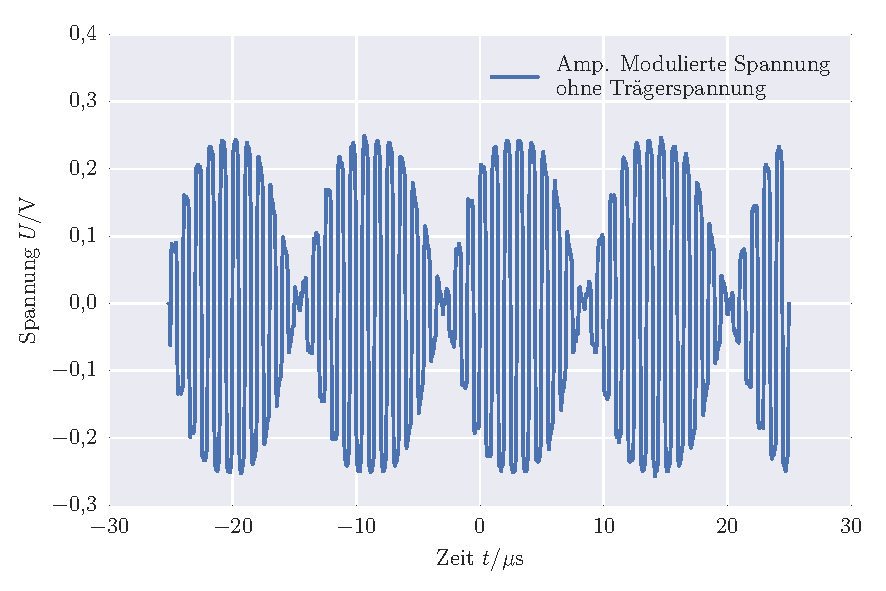
\includegraphics[scale=1]{../Grafiken/Amplituden_Modulierte_Spannung_ohne_Traeger.pdf}
\caption{Ergebnisspannung der Amplitudenmodulation mit Trägerunterdrückung. \label{fig:amplituden_modulierte_spannung_ohne_traeger}}
\end{figure}
\FloatBarrier


\FloatBarrier\begin{figure}[!h]
\centering
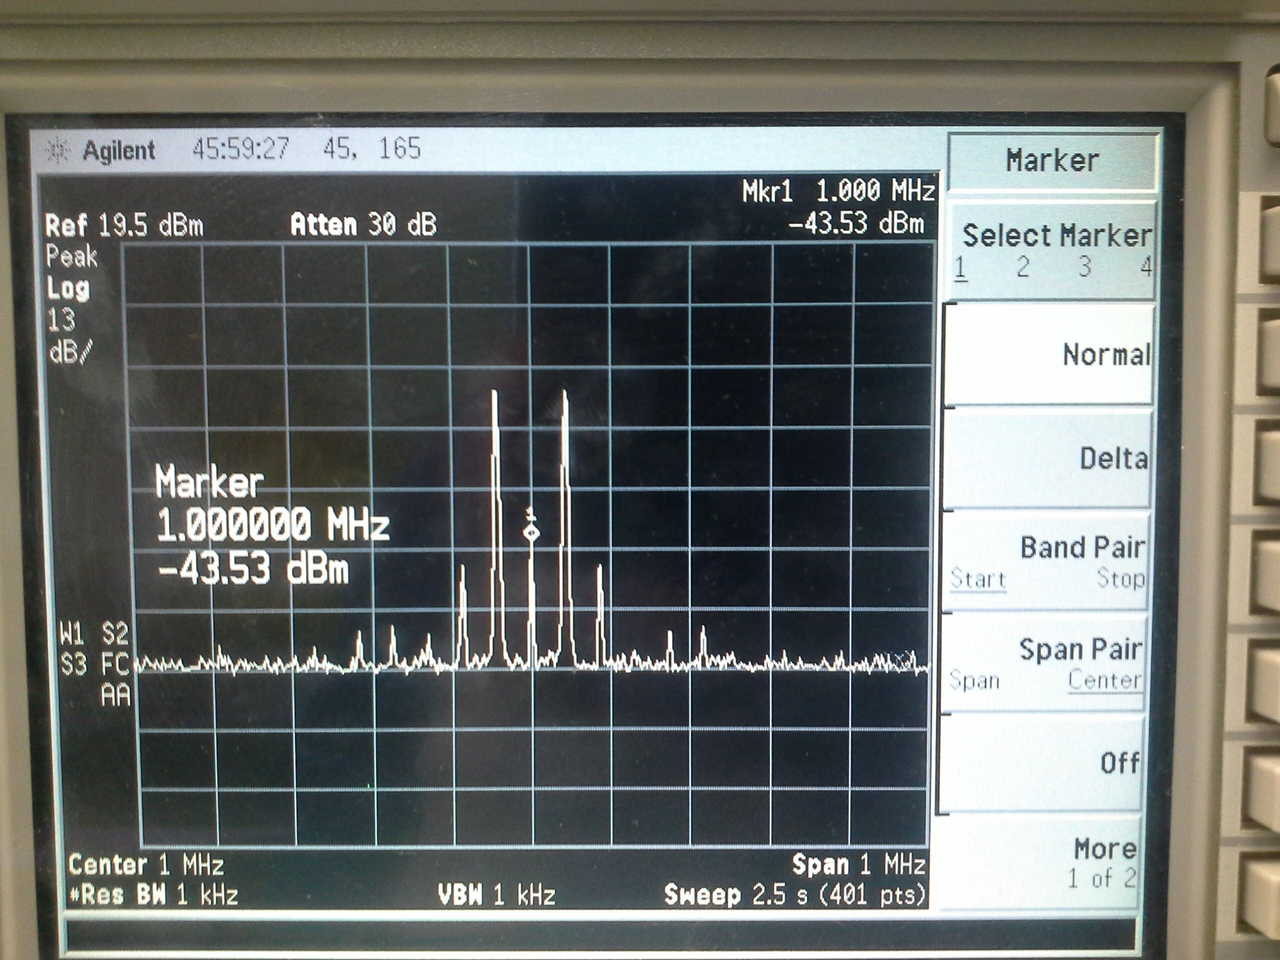
\includegraphics[scale=0.25]{../Grafiken/Frequenzspektrum_b_AmpModuliertTraegerunterdrueckung_0.jpg}
\caption{\label{fig:frequenzspektrum_b_ampmodulierttraegerunterdrueckung_0}}
\end{figure}
\FloatBarrier


\FloatBarrier\begin{figure}[!h]
\centering
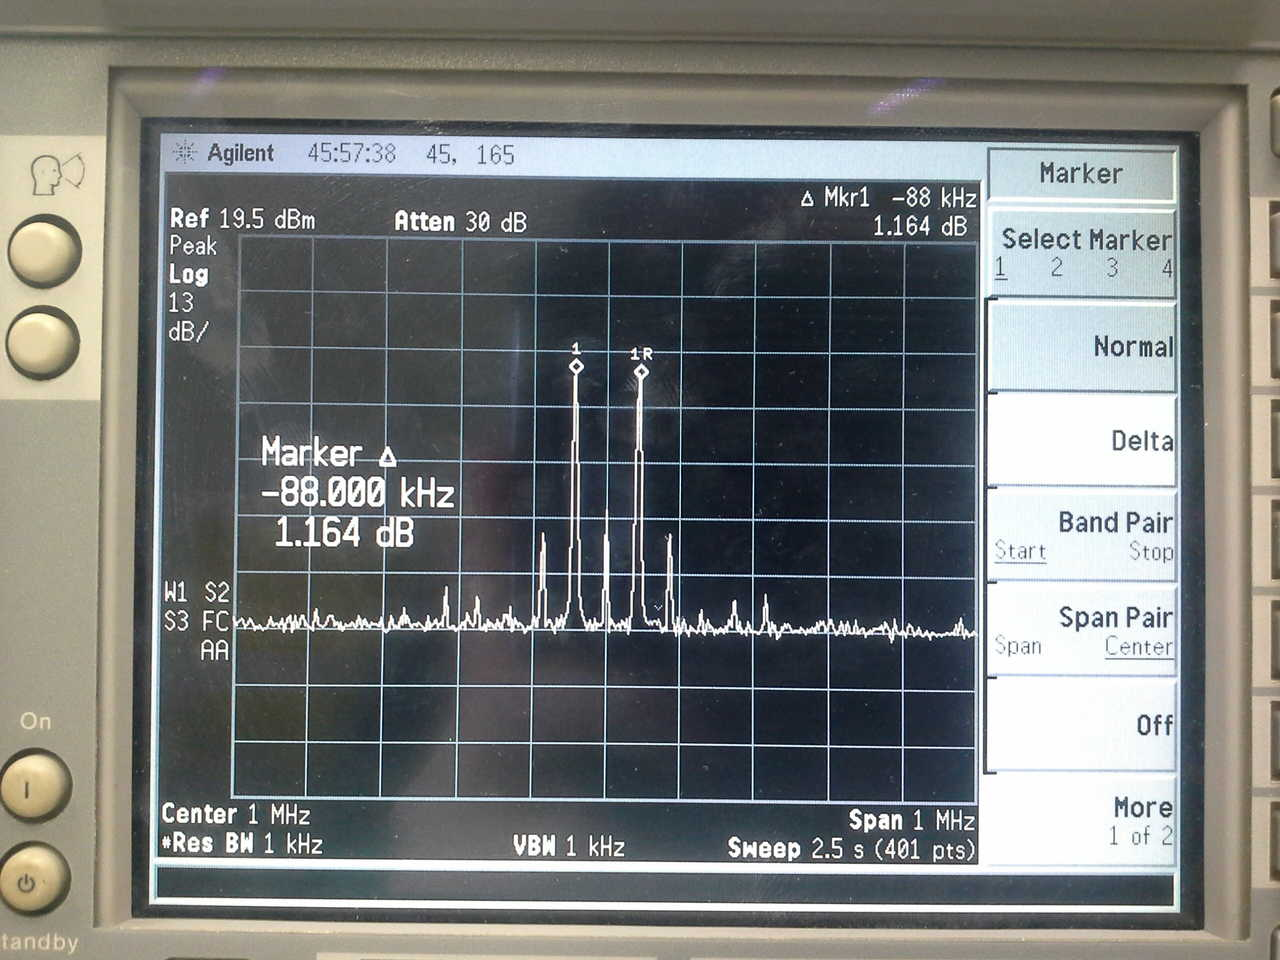
\includegraphics[scale=0.25]{../Grafiken/Frequenzspektrum_b_AmpModuliertTraegerunterdrueckung_1.jpg}
\caption{\label{fig:frequenzspektrum_b_ampmodulierttraegerunterdrueckung_1}}
\end{figure}
\FloatBarrier


\FloatBarrier\begin{figure}[!h]
\centering
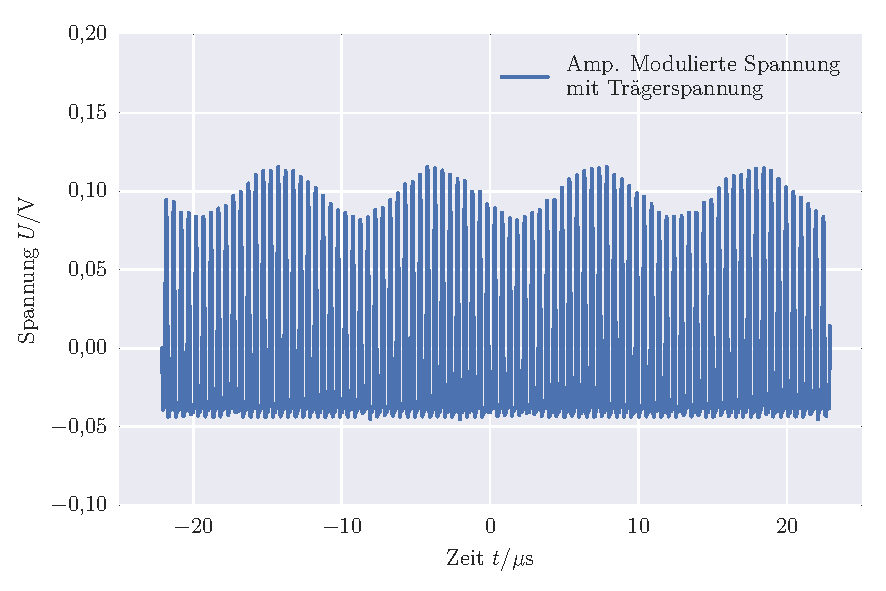
\includegraphics[scale=1]{../Grafiken/Amplituden_Modulierte_Spannung_mit_Traeger.pdf}
\caption{\label{fig:amplituden_modulierte_spannung_mit_traeger}}
\end{figure}
\FloatBarrier


\FloatBarrier\begin{figure}[!h]
\centering
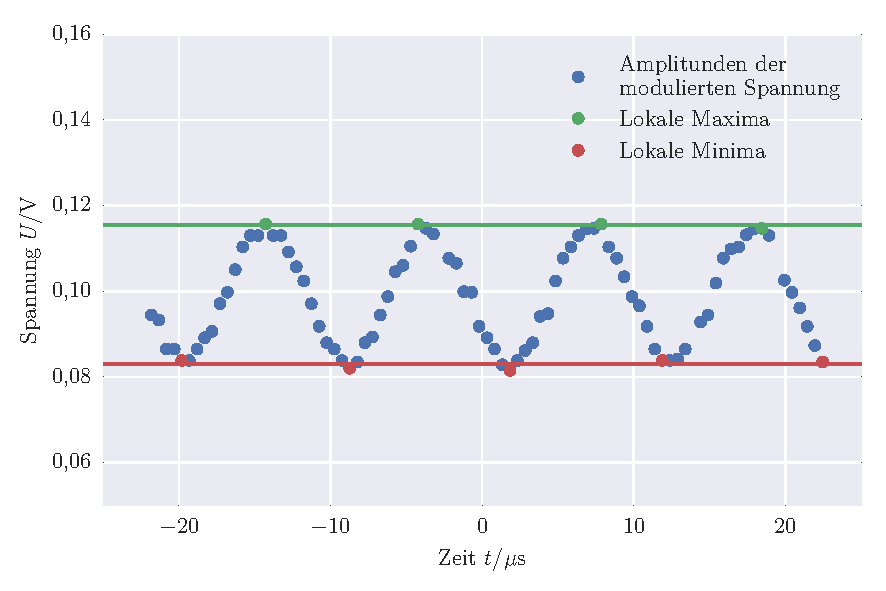
\includegraphics[scale=1]{../Grafiken/Amplituden_Modulierte_Spannung_mit_Traeger_Modulationsgrad.pdf}
\caption{Amplituden der amplitudenmodulierten Spannung aus \cref{fig:amplituden_modulierte_spannung_mit_traeger}.
Farblich hervorgehoben sind jeweils die lokalen Extrema. Die abgebildet Geraden markieren jeweils den Mittelwert
dieser Extremwerte.
 \label{fig:amplituden_modulierte_spannung_mit_traeger_modulationsgrad}}
\end{figure}
\FloatBarrier


\FloatBarrier\begin{figure}[!h]
\centering
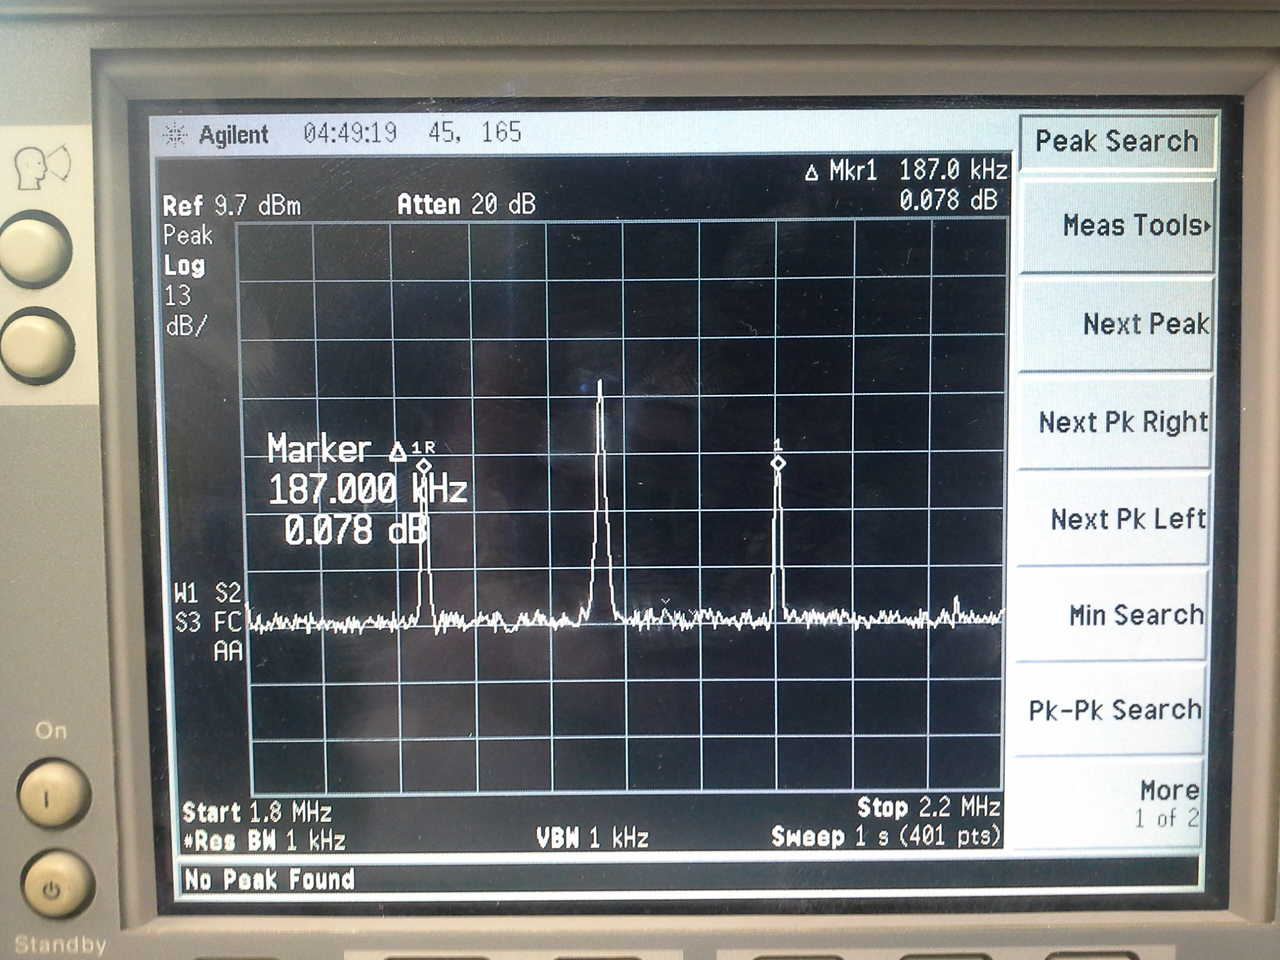
\includegraphics[scale=1]{../Grafiken/Frequenzspektrum_c_AmpModuliertTraeger.jpg}
\caption{\label{fig:frequenzspektrum_c_ampmodulierttraeger}}
\end{figure}
\FloatBarrier


\FloatBarrier\begin{figure}[!h]
\centering
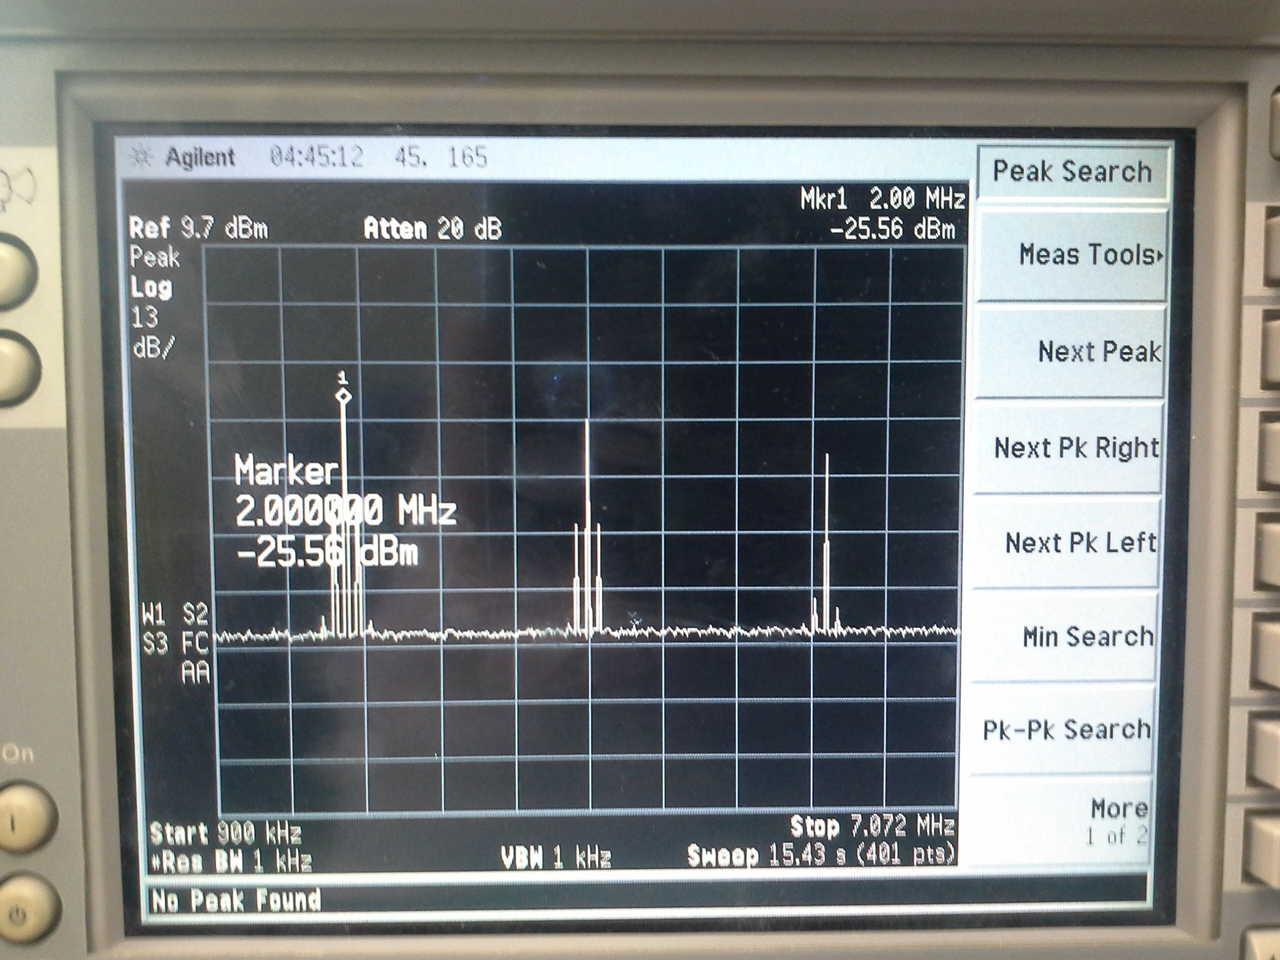
\includegraphics[scale=1]{../Grafiken/Frequenzspektrum_c_AmpModuliertTraeger_Oberwellen_0.jpg}
\caption{\label{fig:frequenzspektrum_c_ampmodulierttraeger_oberwellen_0}}
\end{figure}
\FloatBarrier


\FloatBarrier\begin{figure}[!h]
\centering
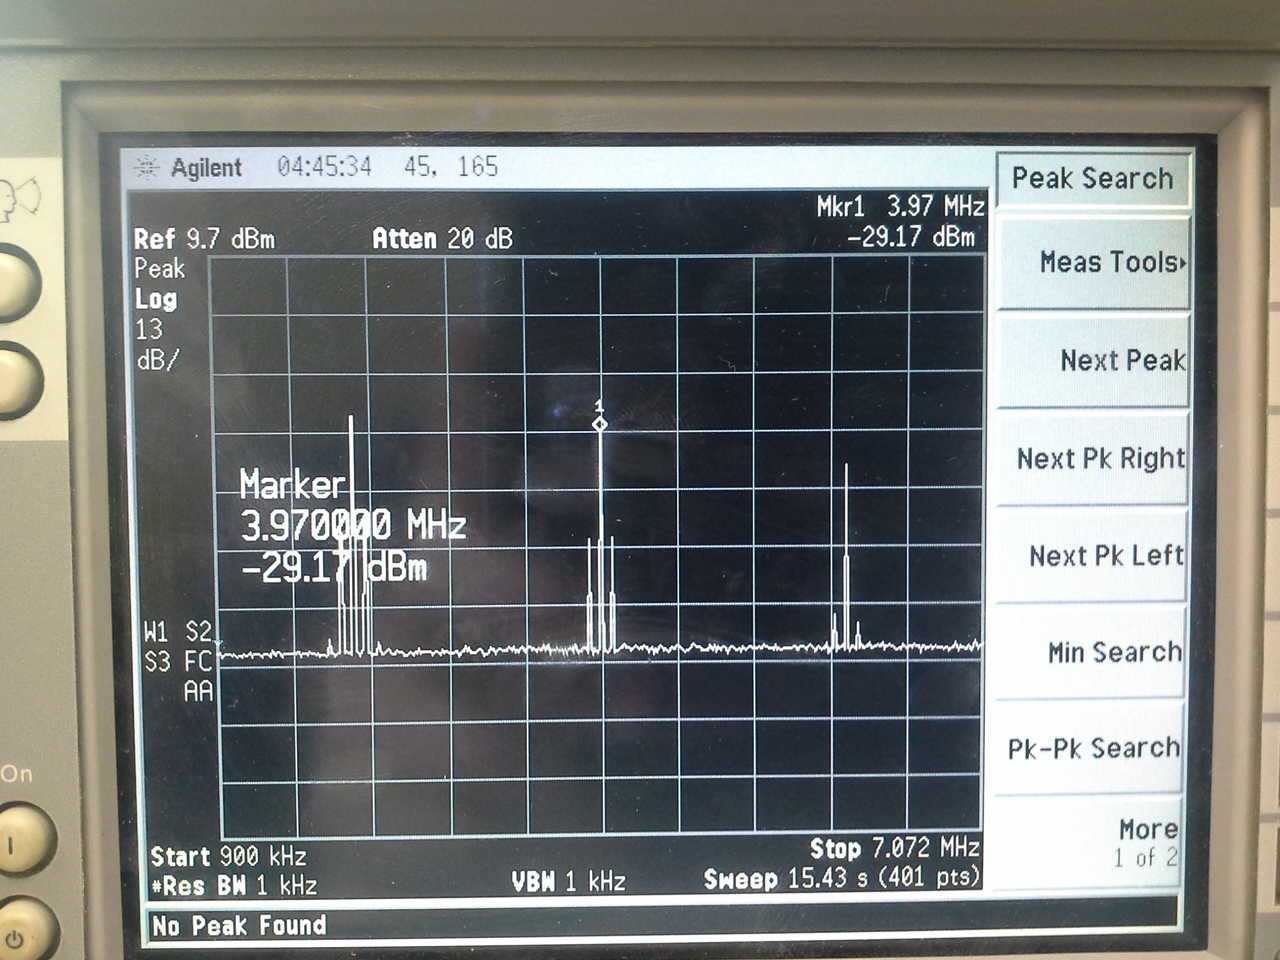
\includegraphics[scale=1]{../Grafiken/Frequenzspektrum_c_AmpModuliertTraeger_Oberwellen_1.jpg}
\caption{\label{fig:frequenzspektrum_c_ampmodulierttraeger_oberwellen_1}}
\end{figure}
\FloatBarrier

\subsection{Demodulation von Amplitudenmodulierten Spannungen}


\FloatBarrier\begin{figure}[!h]
\centering
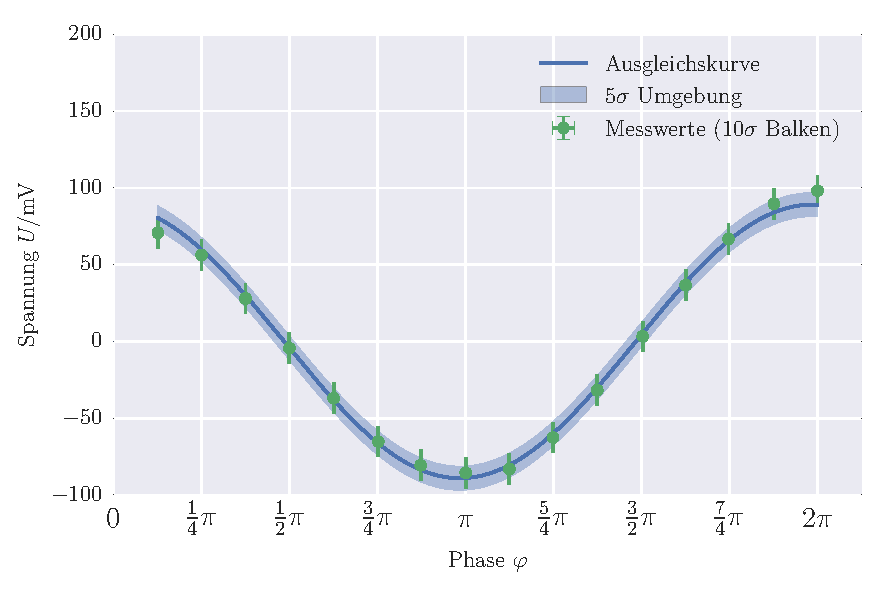
\includegraphics[scale=1]{../Grafiken/Phasenempfindlicher_Gleichrichter.pdf}
\caption{Darstellung der Abhängigkeit der Ausgangs-Gleichspannung des 
	Ringmodulators von der Phase $\varphi$ der Eingangs-Wechselspannungen. 
	Die Fehler der Messwerte sind aufgrund ihres geringen Wertes verzehnfacht
	dargestellt. Und auch das Fehlerband der Ausgleichskurve wurde mit fünf skaliert,
	um sichtbar zu sein.
	\label{fig:phasenempfindlicher_gleichrichter}}
\end{figure}
\FloatBarrier


\FloatBarrier\begin{figure}[!h]
\centering
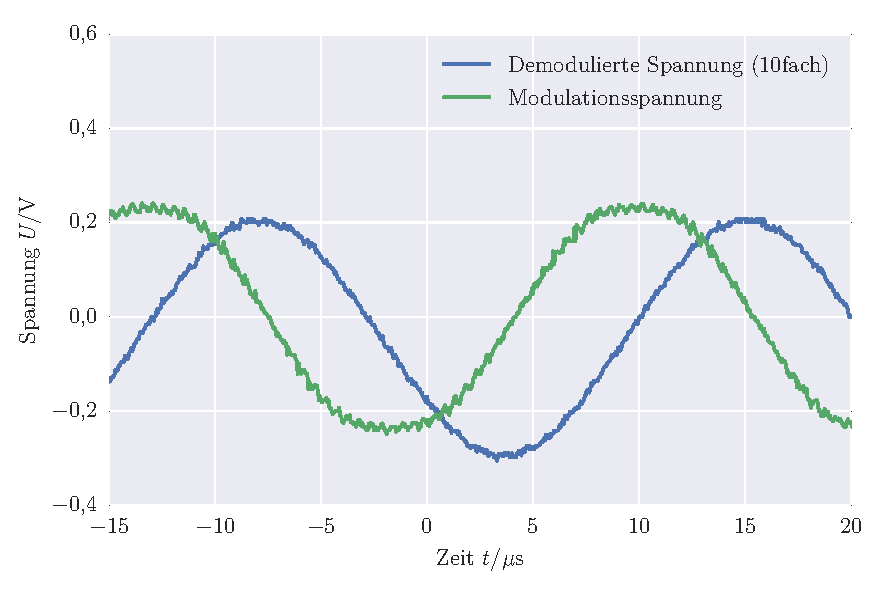
\includegraphics[scale=1]{../Grafiken/Amplituden_Modulation_Ring_Demodulation.pdf}
\caption{\label{fig:amplituden_modulation_ring_demodulation}}
\end{figure}
\FloatBarrier

\FloatBarrier
\begin{figure}[!h]
\centering
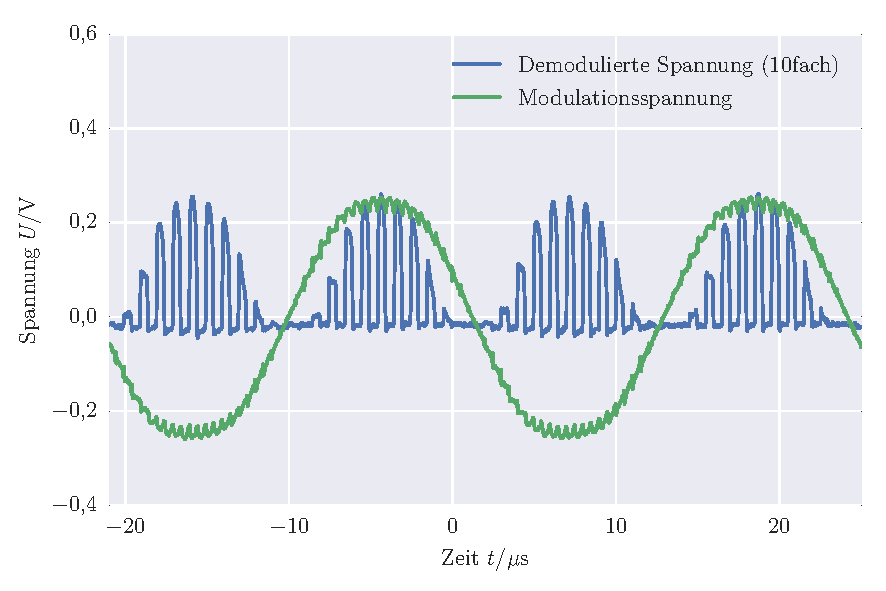
\includegraphics[scale=1]{../Grafiken/Amplituden_Modulation_Diode_Demodulation_Gleichrichter.pdf}
\caption{Spannung die in der Demodulationsschaltung mit Diode nach ebendieser abgegriffen wurde.
	Zu erkennen ist, dass die unteren Halbwellen der modulierten Eingangsspannung durch die Diode
	unterdrückt werden. Der Vergleich mit der Modulationsspannung zeigt das die übrig gebliebenen 
	oberen Halbwellen ihre Amplitude mit der Modulationsfrequenz verändern.   
	\label{fig:amplituden_modulation_diode_demodulation_gleichrichter}}
\end{figure}
\FloatBarrier

\FloatBarrier\begin{figure}[!h]
\centering
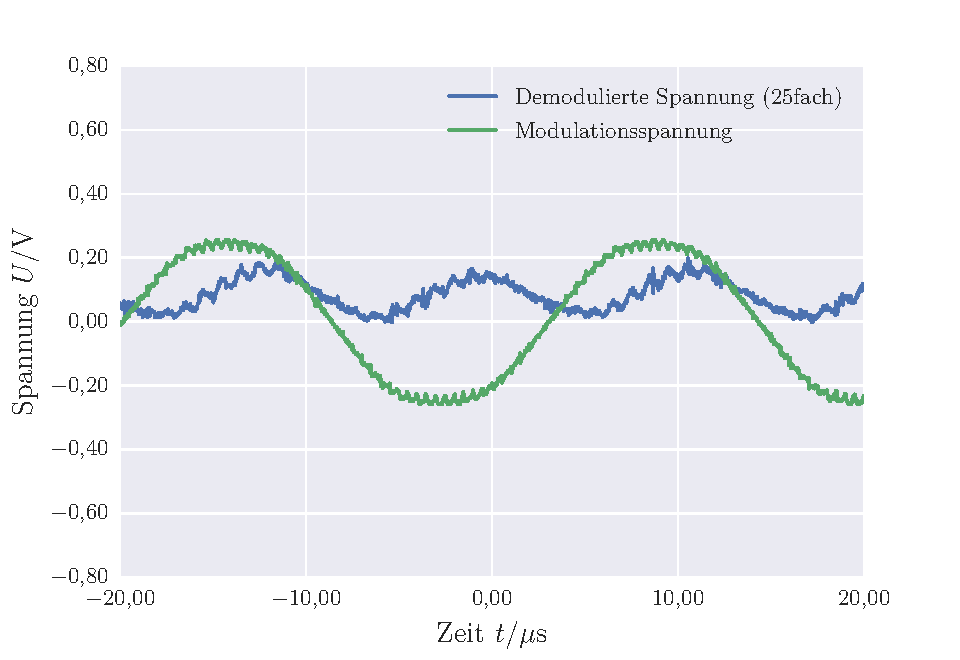
\includegraphics[scale=1]{../Grafiken/Amplituden_Modulation_Diode_Demodulation_Tiefpass.pdf}
\caption{Ergebnisspannung nach Demodulation mit einer Diode und Unterdrückung höherer Frequenzen mit 
	einem Tiefpass. Im Vergleich zur Modulationsfrequenz wird ersichtlich, dass man diese nach der
	Demodulation in abgeschwächter Form und Phasenverschoben zurückerhält.
	  \label{fig:amplituden_modulation_diode_demodulation_tiefpass}}
\end{figure}
\FloatBarrier



\subsection{Frequenzmodulation von Spannungen}

\FloatBarrier\begin{figure}[!h]
\centering
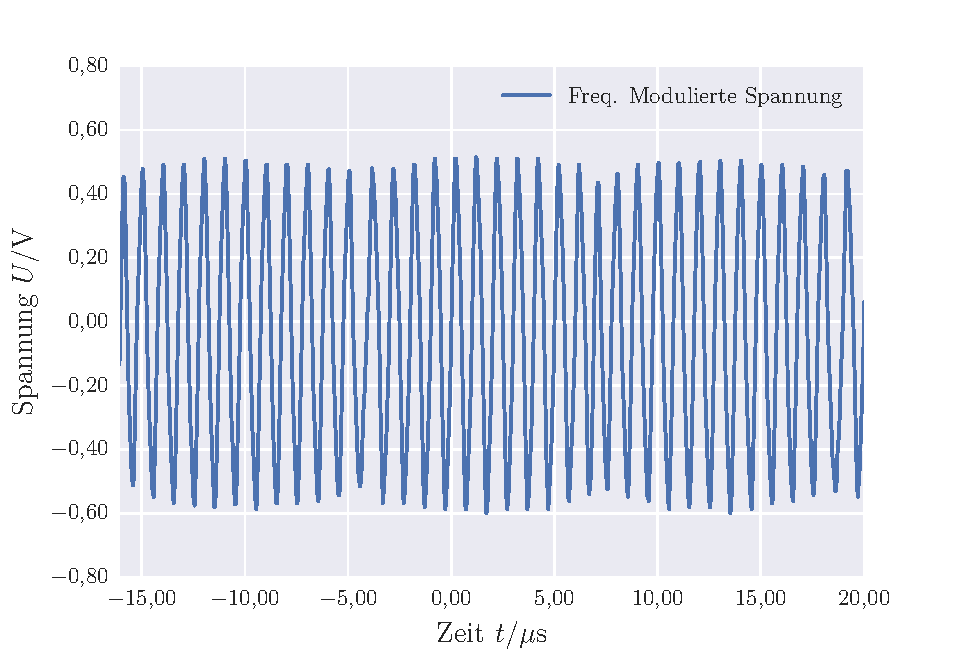
\includegraphics[scale=1]{../Grafiken/Frequenz_Modulierte_Spannung.pdf}
\caption{Frequenzmodulierte Spannung die durch Addition der Seitenbänder aus einer Amplitudenmodulation
	mit Trägerunterdrückung und der phasenverschobenen Trägerspannung erzeugt wurde. Neben der schwachen 
	Frequenzmodulation ist zusätzlich eine geringe Amplitudenmodulation festzustellen.  \label{fig:frequenz_modulierte_spannung}}
\end{figure}
\FloatBarrier

\FloatBarrier\begin{figure}[!h]
\centering
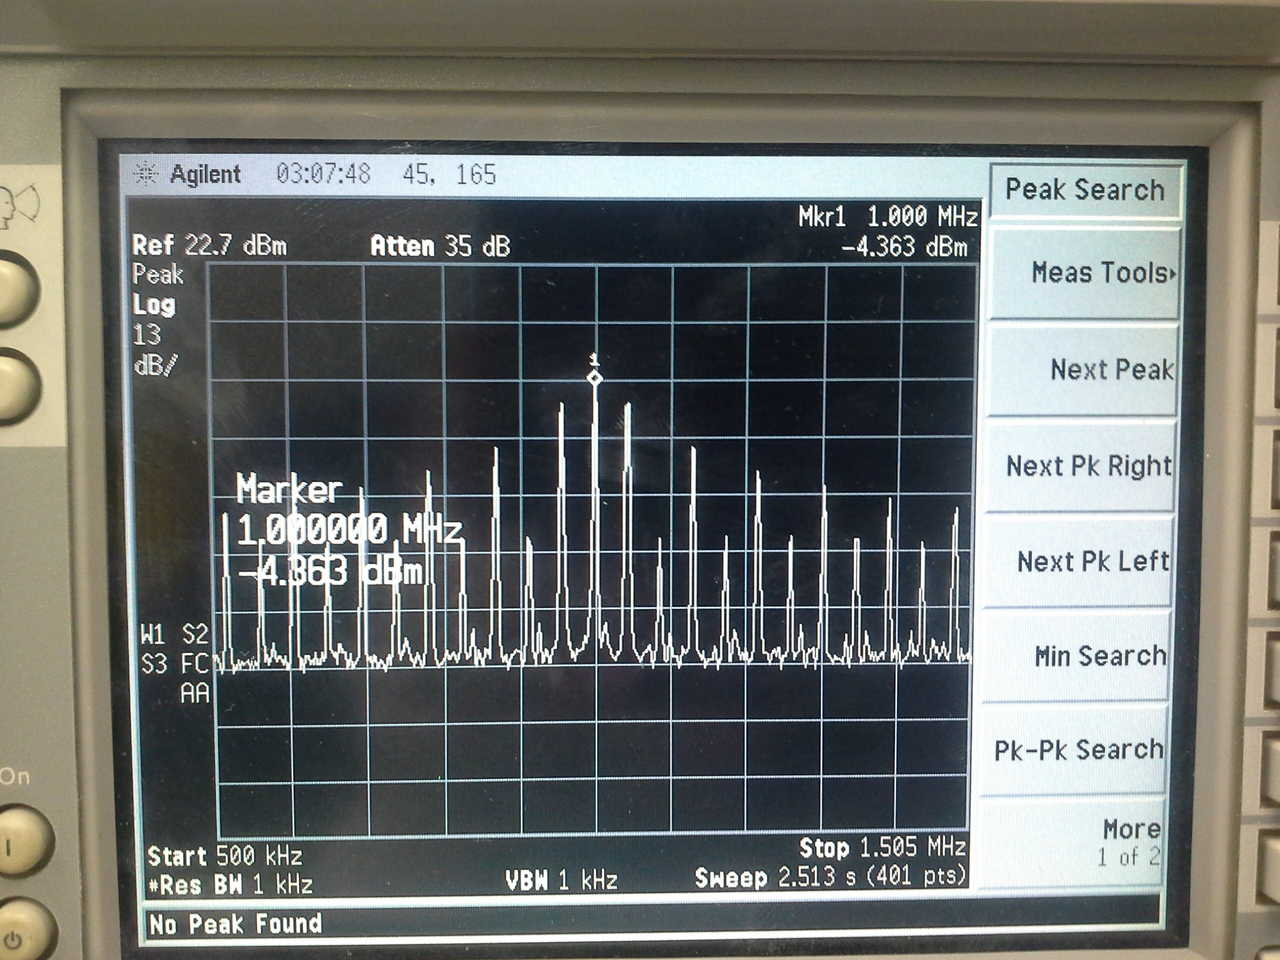
\includegraphics[scale=1]{../Grafiken/Frequenzspektrum_d_FreqModuliert_0.jpg}
\caption{\label{fig:frequenzspektrum_d_freqmoduliert_0}}
\end{figure}
\FloatBarrier

\FloatBarrier\begin{figure}[!h]
\centering
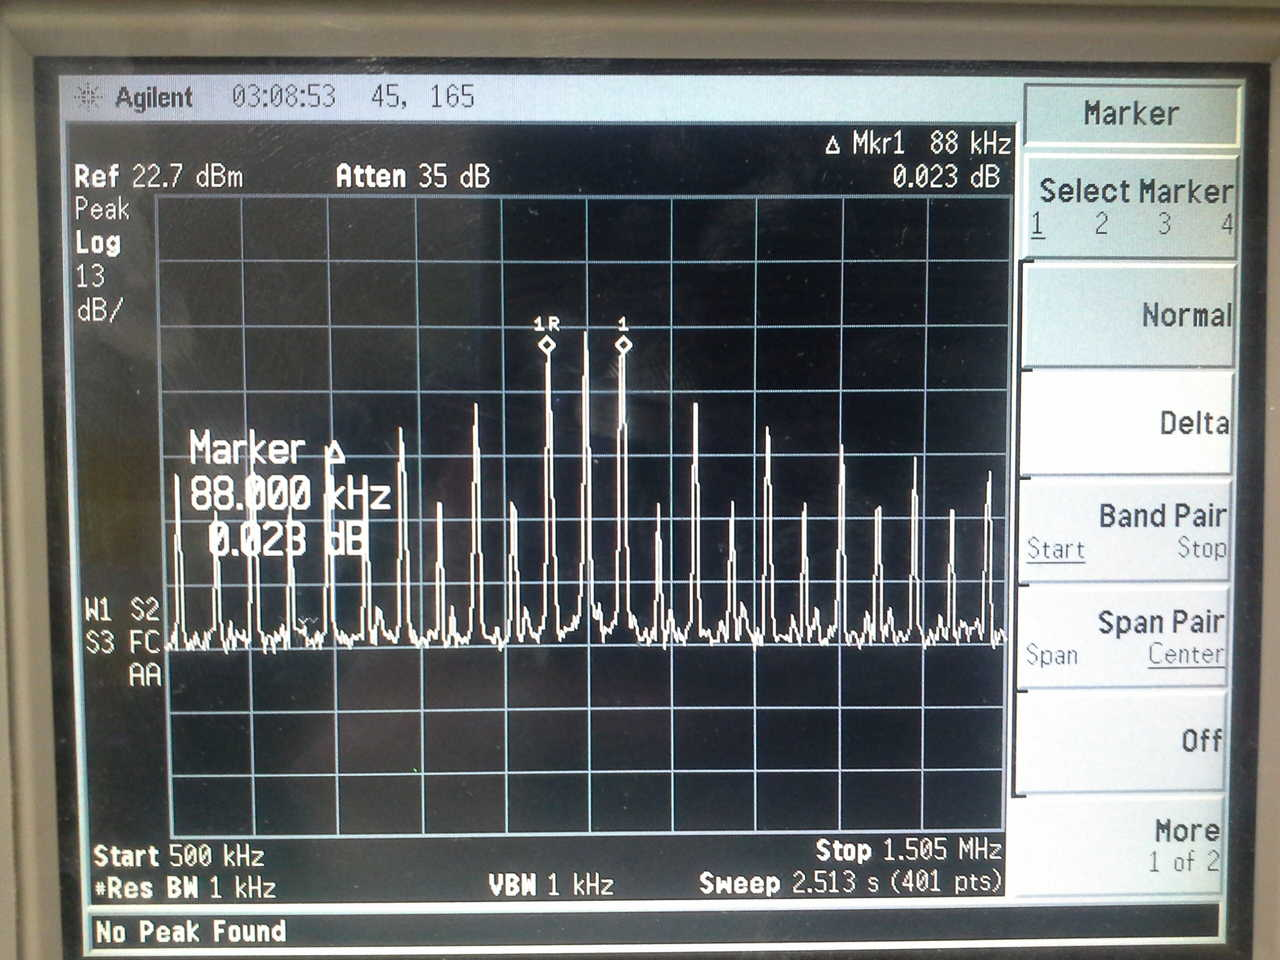
\includegraphics[scale=1]{../Grafiken/Frequenzspektrum_d_FreqModuliert_1.jpg}
\caption{\label{fig:frequenzspektrum_d_freqmoduliert_1}}
\end{figure}
\FloatBarrier

\FloatBarrier\begin{figure}[!h]
\centering
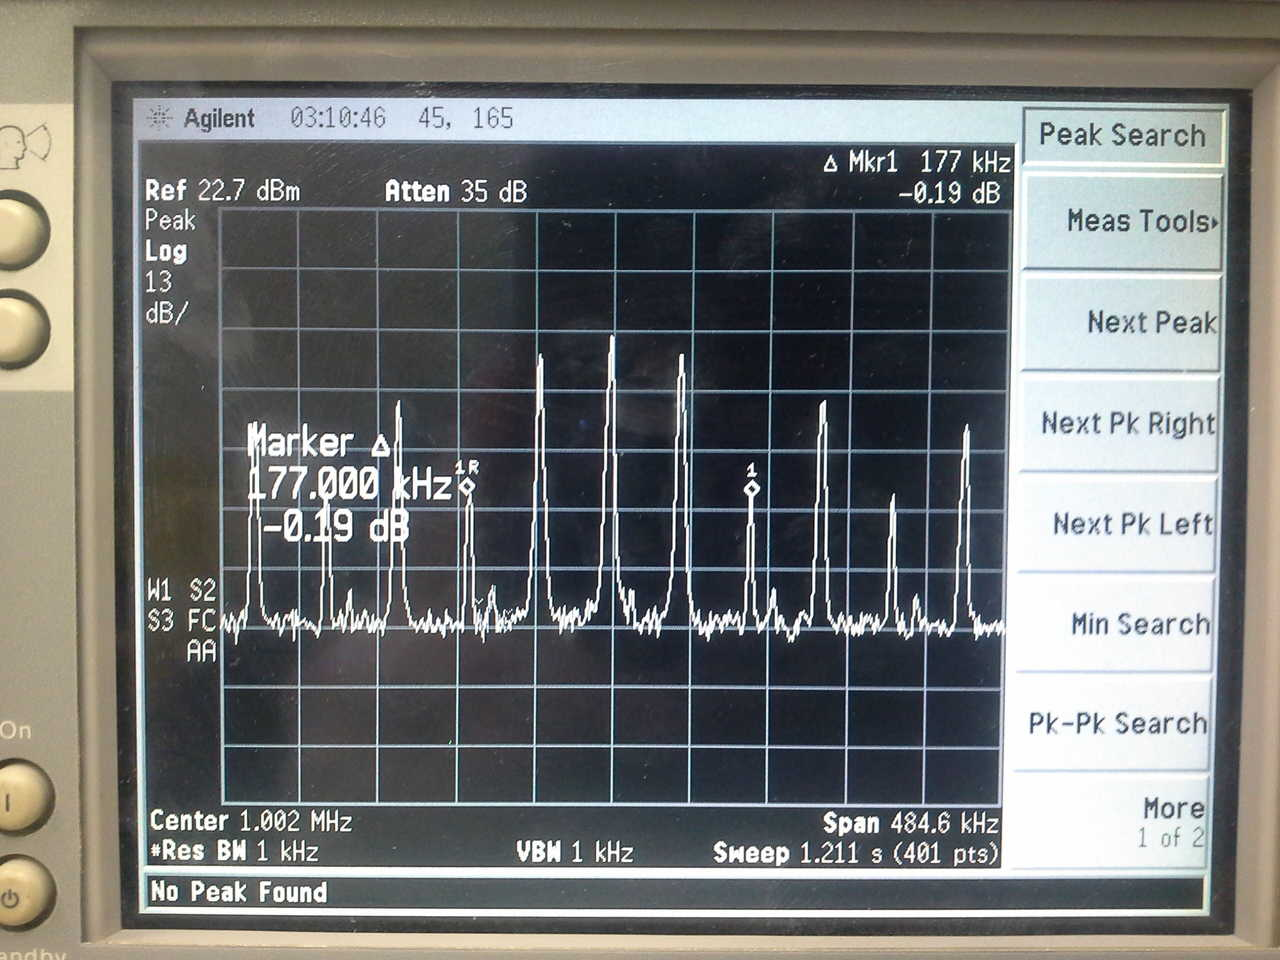
\includegraphics[scale=0.25]{../Grafiken/Frequenzspektrum_d_FreqModuliert_2.jpg}
\caption{\label{fig:frequenzspektrum_d_freqmoduliert_2}}
\end{figure}
\FloatBarrier

\subsection{Demodulation von frequenzmodulierten Spannungen}

\FloatBarrier\begin{figure}[!h]
\centering
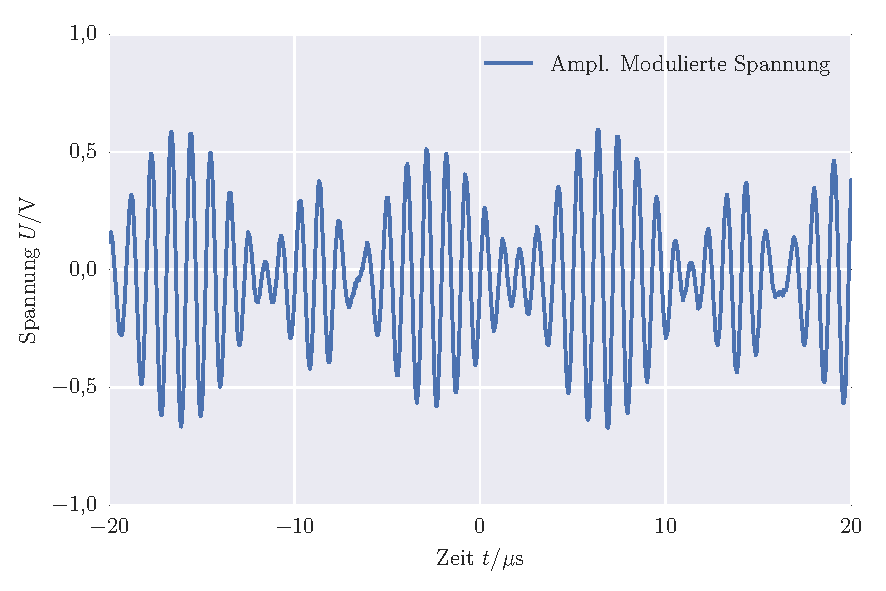
\includegraphics[scale=1]{../Grafiken/Frequenz_Moduliert_Demodulation_Amplitude.pdf}
\caption{Verlauf der amplitudenmodulierten Spannung nach Umwandlung der frequenzmodulierten Spannung durch
	einen Schwingkreis. Anhand des Abweichungen des Verlaufs von einer Schwebung ist zu erkennen, 
	dass weitere Frequenzen neben der Modulationsfrequenz zur Amplitudenmodulation beitragen.   \label{fig:frequenz_moduliert_demodulation_amplitude}}
\end{figure}
\FloatBarrier

\FloatBarrier\begin{figure}[!h]
\centering
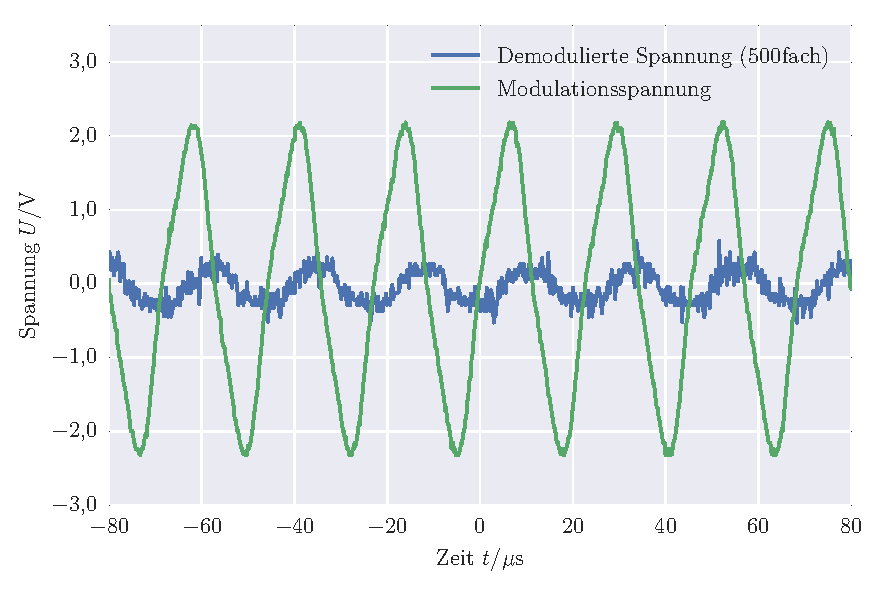
\includegraphics[scale=1]{../Grafiken/Frequenz_Moduliert_Demodulation.pdf}
\caption{\label{fig:frequenz_moduliert_demodulation}}
\end{figure}
\FloatBarrier
